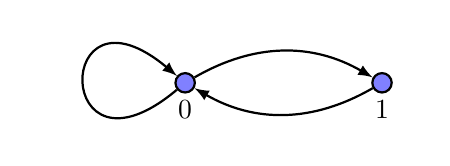
\begin{tikzpicture}[>=latex]
    \clip (-2, -0.7) rectangle (3, 0.7);
    
    \tikzstyle{vert} = [circle, draw, thick, fill = blue!50, inner sep = 0pt, minimum size = 7pt]

    \node[vert] (a) at (0, 0) {};
    \node[below = 3pt] at (a) {$0$};

    \node[vert] (b) at (2.5, 0) {};
    \node[below = 3pt] at (b) {$1$};

    \draw[->, thick] (a) to[out = 220,in = 140, loop, looseness = 30] (a);
    \draw[->, thick] (a) to[bend left] (b);
    \draw[->, thick] (b) to[bend left] (a);
\end{tikzpicture}